% Options for packages loaded elsewhere
\PassOptionsToPackage{unicode}{hyperref}
\PassOptionsToPackage{hyphens}{url}
%
\documentclass[
]{ltjarticle}
\usepackage{lmodern}
\usepackage{amssymb,amsmath}
\usepackage{ifxetex,ifluatex}
\ifnum 0\ifxetex 1\fi\ifluatex 1\fi=0 % if pdftex
  \usepackage[T1]{fontenc}
  \usepackage[utf8]{inputenc}
  \usepackage{textcomp} % provide euro and other symbols
\else % if luatex or xetex
  \usepackage{unicode-math}
  \defaultfontfeatures{Scale=MatchLowercase}
  \defaultfontfeatures[\rmfamily]{Ligatures=TeX,Scale=1}
\fi
% Use upquote if available, for straight quotes in verbatim environments
\IfFileExists{upquote.sty}{\usepackage{upquote}}{}
\IfFileExists{microtype.sty}{% use microtype if available
  \usepackage[]{microtype}
  \UseMicrotypeSet[protrusion]{basicmath} % disable protrusion for tt fonts
}{}
\makeatletter
\@ifundefined{KOMAClassName}{% if non-KOMA class
  \IfFileExists{parskip.sty}{%
    \usepackage{parskip}
  }{% else
    \setlength{\parindent}{0pt}
    \setlength{\parskip}{6pt plus 2pt minus 1pt}}
}{% if KOMA class
  \KOMAoptions{parskip=half}}
\makeatother
\usepackage{xcolor}
\IfFileExists{xurl.sty}{\usepackage{xurl}}{} % add URL line breaks if available
\IfFileExists{bookmark.sty}{\usepackage{bookmark}}{\usepackage{hyperref}}
\hypersetup{
  pdftitle={PDFの変換例},
  pdfauthor={@p1ass},
  hidelinks,
  pdfcreator={LaTeX via pandoc}}
\urlstyle{same} % disable monospaced font for URLs
\usepackage[margin=1in]{geometry}
\usepackage{color}
\usepackage{fancyvrb}
\newcommand{\VerbBar}{|}
\newcommand{\VERB}{\Verb[commandchars=\\\{\}]}
\DefineVerbatimEnvironment{Highlighting}{Verbatim}{commandchars=\\\{\}}
% Add ',fontsize=\small' for more characters per line
\newenvironment{Shaded}{}{}
\newcommand{\AlertTok}[1]{\textcolor[rgb]{1.00,0.00,0.00}{\textbf{#1}}}
\newcommand{\AnnotationTok}[1]{\textcolor[rgb]{0.38,0.63,0.69}{\textbf{\textit{#1}}}}
\newcommand{\AttributeTok}[1]{\textcolor[rgb]{0.49,0.56,0.16}{#1}}
\newcommand{\BaseNTok}[1]{\textcolor[rgb]{0.25,0.63,0.44}{#1}}
\newcommand{\BuiltInTok}[1]{#1}
\newcommand{\CharTok}[1]{\textcolor[rgb]{0.25,0.44,0.63}{#1}}
\newcommand{\CommentTok}[1]{\textcolor[rgb]{0.38,0.63,0.69}{\textit{#1}}}
\newcommand{\CommentVarTok}[1]{\textcolor[rgb]{0.38,0.63,0.69}{\textbf{\textit{#1}}}}
\newcommand{\ConstantTok}[1]{\textcolor[rgb]{0.53,0.00,0.00}{#1}}
\newcommand{\ControlFlowTok}[1]{\textcolor[rgb]{0.00,0.44,0.13}{\textbf{#1}}}
\newcommand{\DataTypeTok}[1]{\textcolor[rgb]{0.56,0.13,0.00}{#1}}
\newcommand{\DecValTok}[1]{\textcolor[rgb]{0.25,0.63,0.44}{#1}}
\newcommand{\DocumentationTok}[1]{\textcolor[rgb]{0.73,0.13,0.13}{\textit{#1}}}
\newcommand{\ErrorTok}[1]{\textcolor[rgb]{1.00,0.00,0.00}{\textbf{#1}}}
\newcommand{\ExtensionTok}[1]{#1}
\newcommand{\FloatTok}[1]{\textcolor[rgb]{0.25,0.63,0.44}{#1}}
\newcommand{\FunctionTok}[1]{\textcolor[rgb]{0.02,0.16,0.49}{#1}}
\newcommand{\ImportTok}[1]{#1}
\newcommand{\InformationTok}[1]{\textcolor[rgb]{0.38,0.63,0.69}{\textbf{\textit{#1}}}}
\newcommand{\KeywordTok}[1]{\textcolor[rgb]{0.00,0.44,0.13}{\textbf{#1}}}
\newcommand{\NormalTok}[1]{#1}
\newcommand{\OperatorTok}[1]{\textcolor[rgb]{0.40,0.40,0.40}{#1}}
\newcommand{\OtherTok}[1]{\textcolor[rgb]{0.00,0.44,0.13}{#1}}
\newcommand{\PreprocessorTok}[1]{\textcolor[rgb]{0.74,0.48,0.00}{#1}}
\newcommand{\RegionMarkerTok}[1]{#1}
\newcommand{\SpecialCharTok}[1]{\textcolor[rgb]{0.25,0.44,0.63}{#1}}
\newcommand{\SpecialStringTok}[1]{\textcolor[rgb]{0.73,0.40,0.53}{#1}}
\newcommand{\StringTok}[1]{\textcolor[rgb]{0.25,0.44,0.63}{#1}}
\newcommand{\VariableTok}[1]{\textcolor[rgb]{0.10,0.09,0.49}{#1}}
\newcommand{\VerbatimStringTok}[1]{\textcolor[rgb]{0.25,0.44,0.63}{#1}}
\newcommand{\WarningTok}[1]{\textcolor[rgb]{0.38,0.63,0.69}{\textbf{\textit{#1}}}}
\usepackage{longtable,booktabs}
% Correct order of tables after \paragraph or \subparagraph
\usepackage{etoolbox}
\makeatletter
\patchcmd\longtable{\par}{\if@noskipsec\mbox{}\fi\par}{}{}
\makeatother
% Allow footnotes in longtable head/foot
\IfFileExists{footnotehyper.sty}{\usepackage{footnotehyper}}{\usepackage{footnote}}
\makesavenoteenv{longtable}
\usepackage{graphicx,grffile}
\makeatletter
\def\maxwidth{\ifdim\Gin@nat@width>\linewidth\linewidth\else\Gin@nat@width\fi}
\def\maxheight{\ifdim\Gin@nat@height>\textheight\textheight\else\Gin@nat@height\fi}
\makeatother
% Scale images if necessary, so that they will not overflow the page
% margins by default, and it is still possible to overwrite the defaults
% using explicit options in \includegraphics[width, height, ...]{}
\setkeys{Gin}{width=\maxwidth,height=\maxheight,keepaspectratio}
% Set default figure placement to htbp
\makeatletter
\def\fps@figure{htbp}
\makeatother
\usepackage[normalem]{ulem}
% Avoid problems with \sout in headers with hyperref
\pdfstringdefDisableCommands{\renewcommand{\sout}{}}
\setlength{\emergencystretch}{3em} % prevent overfull lines
\providecommand{\tightlist}{%
  \setlength{\itemsep}{0pt}\setlength{\parskip}{0pt}}
\setcounter{secnumdepth}{5}
\usepackage{listings}
\usepackage{xcolor}
 
\lstset{
    basicstyle=\ttfamily,
    keywordstyle=\color[RGB]{33,74,135}\bfseries,
    stringstyle=\color[RGB]{79,153,5},
    commentstyle=\color[RGB]{143,89,2}\itshape,
    numberstyle=\footnotesize,
    numbers=left,
    stepnumber=1,
    numbersep=15pt,
    backgroundcolor=\color[RGB]{251,251,251},
    frame=single,
    frameround=ffff,
    framesep=5pt,
    rulecolor=\color[RGB]{148,150,152}, 
    breaklines=true,
    breakautoindent=true,
    breakatwhitespace=true,
    breakindent=25pt,
    showspaces=false,
    showstringspaces=false,
    showtabs=false,
    tabsize=2,
    captionpos=b,
    linewidth=\textwidth,
}

\title{PDFの変換例}
\author{@p1ass}
\date{\the\year/\the\month/\the\day}

\begin{document}
\maketitle

\hypertarget{ux76eeux7684}{%
\section{目的}\label{ux76eeux7684}}

PDFに変換できるマークダウンの記法を学ぶ。

\hypertarget{ux898bux51faux3057}{%
\section{見出し}\label{ux898bux51faux3057}}

\hypertarget{h2ux898bux51faux3057}{%
\subsection{h2見出し}\label{h2ux898bux51faux3057}}

\hypertarget{ux30a4ux30f3ux30e9ux30a4ux30f3ux6570ux5f0f}{%
\subsubsection{インライン数式}\label{ux30a4ux30f3ux30e9ux30a4ux30f3ux6570ux5f0f}}

インライン数式はドル記号\texttt{\$}で囲って、
\(V = R \times I\)のようにTeXと同じ書き方で書くことができる。

\hypertarget{ux756aux53f7ux4ed8ux304dux30c7ux30a3ux30b9ux30d7ux30ecux30a4ux6570ux5f0fux30e2ux30fcux30c9}{%
\subsubsection{番号付きディスプレイ数式モード}\label{ux756aux53f7ux4ed8ux304dux30c7ux30a3ux30b9ux30d7ux30ecux30a4ux6570ux5f0fux30e2ux30fcux30c9}}

数式ブロックはドル記号2つ\texttt{\$\$}で囲む。\texttt{\{\#eq:equation\}}を最後につけることでラベルを貼れる。
参照は\texttt{{[}@eq:equation{]}}のように書くことができる。

不純物濃度の深さ方向分布は式~\ref{eq:equation}の拡散方程式を解くことで得られる。

\begin{equation}
\frac{\partial N(x,t)}{\partial t} = D \frac{\partial^2N(x,t)}{\partial x^2}
\label{eq:equation}\end{equation}

また、\texttt{\textbackslash{}begin\{eqnarray\}}が使えるので、イコールを揃える時はこちらを使うと良い。

\begin{eqnarray}
x + y &=& 5 \label{easy_eq} \\
x &=& 2
\end{eqnarray}

式\ref{easy_eq}を解くと、\(y = 3\)が得られる。

\hypertarget{texux30b3ux30deux30f3ux30c9}{%
\section{texコマンド}\label{texux30b3ux30deux30f3ux30c9}}

一度\texttt{.tex}ファイルに変換してからPDFに変換するので、texのコマンドも使用できる。
例えば、\texttt{\textbackslash{}clearpage}を使うことで改ページができる。

改ページ前↑

\clearpage

改ページ後↓

\hypertarget{ux753bux50cf}{%
\section{画像}\label{ux753bux50cf}}

画像はマークダウンと同じ記法で書くことができる。文末に\texttt{\{\#fig:LABEL\}}とすることでラベルを付与できる。\texttt{\{\#fig:LABEL\ height=100mm\}}とすることで、画像の大きさも調整できる。

\begin{figure}
\hypertarget{fig:solar}{%
\centering
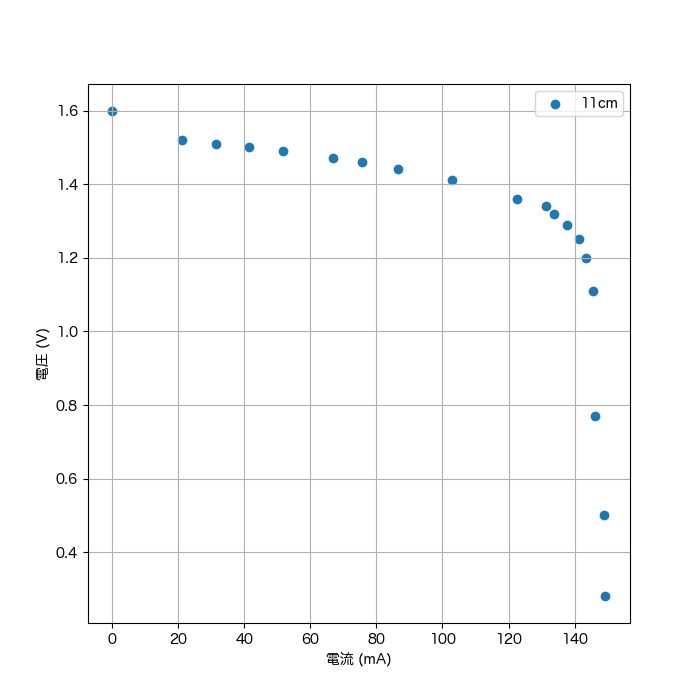
\includegraphics[width=\textwidth,height=100mm]{solar.png}
\caption{太陽電池の出力特性}\label{fig:solar}
}
\end{figure}

\texttt{{[}@fig:LABEL{]}}とすることで、参照を貼れる。

太陽電池の出力特性を図~\ref{fig:solar}に示す。

\hypertarget{ux8868}{%
\section{表}\label{ux8868}}

表のタイトル、ラベルは\texttt{:タイトル\ \{\#tbl:LABEL\}}のように書くことができる。

\hypertarget{tbl:table}{}
\begin{longtable}[]{@{}cr@{}}
\caption{\label{tbl:table}標本化周波数を変えたときの観測周波数の変化}\tabularnewline
\toprule
標本化周波数 \(\mathrm{(kSa/s)}\) & 観測周波数
\(\mathrm{(kHz)}\)\tabularnewline
\midrule
\endfirsthead
\toprule
標本化周波数 \(\mathrm{(kSa/s)}\) & 観測周波数
\(\mathrm{(kHz)}\)\tabularnewline
\midrule
\endhead
100 & 6.1\tabularnewline
250 & 53\tabularnewline
500 & 100\tabularnewline
1000 & 100\tabularnewline
\bottomrule
\end{longtable}

表への参照を貼る時は\texttt{{[}@tbl:LABEL{]}}のように書く。

標本化周波数を変えたときの観測周波数の変化を表~\ref{tbl:table}に示す。

\hypertarget{sec:section}{%
\subsection{セクション参照}\label{sec:section}}

\texttt{{[}@sec:LABEL{]}}と書くことでセクションを参照できる。

節~\ref{sec:section}によると、セクションの参照も可能である。

\hypertarget{ux6ce8ux91c8}{%
\section{注釈}\label{ux6ce8ux91c8}}

注釈\footnote{注釈とはほげほげ}

\hypertarget{ux30deux30fcux30afux30c0ux30a6ux30f3ux8a18ux6cd5}{%
\section{マークダウン記法}\label{ux30deux30fcux30afux30c0ux30a6ux30f3ux8a18ux6cd5}}

\begin{itemize}
\tightlist
\item
  箇条書き1

  \begin{itemize}
  \tightlist
  \item
    サブ箇条書き1
  \item
    サブ箇条書き2
  \end{itemize}
\item
  箇条書き2
\item
  箇条書き3
\end{itemize}

\begin{enumerate}
\def\labelenumi{\arabic{enumi}.}
\tightlist
\item
  番号付きリスト1

  \begin{enumerate}
  \def\labelenumii{\arabic{enumii}.}
  \tightlist
  \item
    サブ番号付きリスト1
  \item
    サブ番号付きリスト1
  \end{enumerate}
\item
  番号付きリスト2
\item
  番号付きリスト3
\end{enumerate}

\textbf{太字}

\sout{取り消し線}

水平線

\begin{center}\rule{0.5\linewidth}{\linethickness}\end{center}

\href{https://google.com}{googleへのリンク}

コードブロック

\begin{Shaded}
\begin{Highlighting}[]
\PreprocessorTok{#include }\ImportTok{<stdio.h>}

\DataTypeTok{int}\NormalTok{ main(}\DataTypeTok{void}\NormalTok{) \{}
\NormalTok{    printf(}\StringTok{"Hello World}\SpecialCharTok{\textbackslash{}n}\StringTok{"}\NormalTok{);}
\NormalTok{\}}
\end{Highlighting}
\end{Shaded}

listingsパッケージ

\lstinputlisting[language=c, caption = ソースコード ,label = source]{example.c}

\end{document}
